\begingroup
\renewcommand{\cleardoublepage}{}
\renewcommand{\clearpage}{}
\chapter{État de l'art}
\endgroup

Ce chapitre va s'intéresser en premier lieu à l'hypothèse du stockage sécurisé dans un
environnement cloud. Puis, le chapitre va s'intéresser à de potentielles solutions des challenges posés au niveau de la virtualisation en terme de sécurité. Enfin, on discutera d'une solution garantissant une authentification sécurisée de plusieurs acteurs d’un même système

\section{Stockage}\label{sec:sto}

Le stockage est l'une des trois hypothèses posées dans l'introduction. Pour
pouvoir nous focaliser sur les communications dans un environnement cloud, il
est capital d'établir un schéma avec un stockage sécurisé. Le stockage est un
élément central dans l'environnement cloud. Le cloud n’offre pas tous les
droits à l’utilisateur sur les données. En effet, un utilisateur n'a qu'un
droit de contrôle sur la VM sur laquelle dont il est l'utilisateur. Les
fournisseurs de service de cloud (appelé CSP pour \textit{Cloud Service Provider}), eux, ont le rôle de gérer les données
et les serveurs. Mais, ce niveau de contrôle doit être maîtrisé et vérifié, car
l'environnement cloud (architecture \textit{multi-tenant} et virtualisation) a généré de nouvelles menaces. Le stockage doit faire face différentes menaces : une confidentialité et une intégrité des données non maîtrisées, une vulnérabilité sur la récupération des données (données d'un utilisateur ayant eu la même image précédemment), un mauvais nettoyage des supports (changement de disque nécessaire ou données stockées inutilisées), un \textit{backup} des données non sécurisé, des vulnérabilités via les applications Web (\cite{web_security}) ou encore une authentification et un contrôle d'accès insuffisamment efficace.

Dans cet optique, nous avons suivi les principales recommandations du CSA
(\textit{Cloud Security Alliance}) en terme de gestion des clés et de stockage des données (\cite{security_guidelines}) :
Premièrement, la gestion des clés doit être effectuée par les organisations/utilisateurs eux-mêmes ou bien par un service cryptographique de confiance avec un service crédible et neutre. Deuxièmement, les meilleurs pratiques pour la gestion des clés et de chiffrement provenant de source fiable doivent être utilisées. Troisièmement, il est recommandé d'utiliser une technologie standardisée dans la mesure du possible. Quatrièmement, la portée d'une clé ne doit pas dépasser un utilisateur ou un groupe d'utilisateur. Enfin, l'utilisation d'algorithmes standards est recommandée et les algorithmes de chiffrement propriétaires sont déconseillés.

Sur la base de l'étude \cite{security_cloud_survey}, il en ressort plusieurs solutions. Nous avons décidé d'en retenir deux dans le but d'offrir des approches différentes selon le stockage souhaité. Ces deux solutions ont été choisies, car elles mettent en place les recommandations de sécurité du CSA \cite{security_guidelines}. De plus, les solutions sont présentées dans le papier Mazhar et al \cite{security_cloud_survey} et ont l'avantage d'être des solutions récentes pour sécuriser le stockage dans le cloud : FADE (\cite{fade}), SecCloud (\cite{secCloud}).

\subsection{FADE}

FADE (\textit{File Assured Deletion}) est un protocole permettant une gestion de clés cryptographiques et utilisant des techniques de cryptographie symétriques et asymétriques. Ce protocole garantit une confidentialité et une intégrité des données dans un environnement cloud en fonctionnant avec des groupes de gestion de clés (KM pour \textit{key manager}) agissant comme un \gls{TPA} (\textit{Trusted Party Third}) et générant des clés publiques/privées.
Différents cryptages sur les mêmes données permettent de sécuriser ces dernières et d'effectuer un contrôle d'accès implicite des données. Le fonctionnement du protocole est décrit sur la figure \ref{label-image1} : pour encrypter un fichier F de l'utilisateur, une clé de donnée aléatoire K est utilisée. Ce fichier F, encrypté par K, sera encrypté par une clé symétrique S. Enfin, la paire de clé générée par KM encrypte S. Un ficher de politique d'accès P permet de vérifier qui peut accéder au fichier. 
\newline
Pour télécharger un fichier stocké cloud, un utilisateur doit effectuer une requête en envoyant P auprès du KM afin qu'il lui délivre une paire de clé publique/privée. La clé publique sera transmise à l'utilisateur qui encryptera le fichier F en encryptant F avec K et K avec S. Enfin, la clé publique, délivrée par KM, encryptera S. Le fichier F est stockée dans le cloud avec un haut niveau de cryptage et avec le fichier P. Pour décrypter un fichier stocké dans le cloud, il est nécessaire que l'utilisateur envoie S à KM afin de décrypter le fichier, puis décrypter F. 
\newline
Enfin, un écrasement sécurisé des clés cryptographiques et d'un fichier de politique (politique vis-à-vis des accès au fichier stocké sur le cloud par un utilisateur) permet de rendre les données inaccessibles et donc assurément supprimées.
\newline 
Une solution retenue pour le stockage dans le cloud est FADE, car elle permet un contrôle d'accès et une suppression définitive des données, tout en proposant un scalabilité élevé, un cryptage des données avec l'aide d'un TPA et garantit l'intégrité et la confidentialité des données.

\begin{figure}[hb]
	\center
	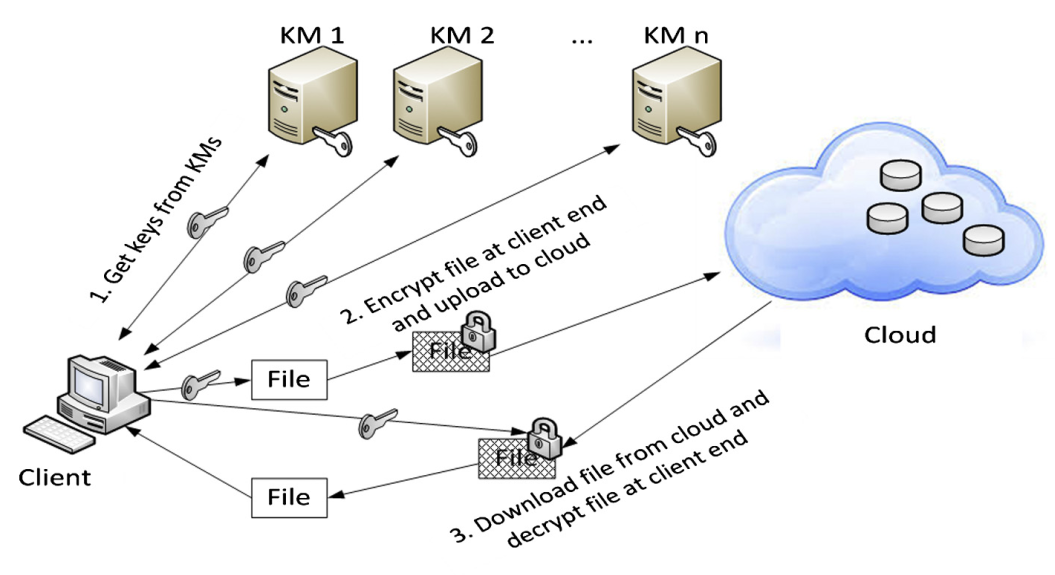
\includegraphics[height=7.5cm]{./pics/schema_fade.png}
	\caption{Fonctionnement du protocole FADE [\cite{security_cloud_survey}]}
	\label{label-image1}
\end{figure}

\subsection{SecCloud}
SecCloud est un protocole cherchant à protéger les données stockées par un utilisateur, mais également les calculs effectués sur ces données. Le protocole se base sur l'utilisation d'une cryptographie à base de couplage pour permettre de générer des clés pour les utilisateurs, le CSP et un TPA. Un utilisateur peut alors stocker ses données dans l'espace de stockage fourni par un CSP et ces données sont signées par un TPA. Les données sont alors envoyées au cloud avec la signature du TPA et encryptées avec une clé de session. Le cloud va alors décrypté ces données, vérifié la signature du TPA et stocké les données dans les partitions désignées dans le but d'empêcher toute violation des données. 
L'algorithme Merkle Hash Tree, reconstruit par le TPA, permet de vérifier les calculs effectués sur les données. Le TPA a une place importante, car il a le devoir de vérifier l’accessibilité et l’intégrité des données sur requête du client.
\newline
SecCloud est une solution pertinente pour le stockage dans le cloud. L'utilisation d'un TPA, la vérification de signature et l'utilisation d'une cryptographie à base de couplage pour crypter les données sont des fonctionnalités alléchantes de cette solution. Elle assure la confidentialité et l'intégrité des données via ces fonctionnalités.

\section{Virtualisation}\label{sec:vir}

La virtualisation permet l’utilisation des mêmes ressources physiques pour
plusieurs utilisateurs. Une VM est instanciée pour chaque utilisateur et permet
alors à l’utilisateur d’avoir une machine complète et opérationnelle. Plusieurs machines virtuelles peuvent être sur les mêmes ressources physiques et créer un environnement multi-tenant.
Tout comme le stockage, la virtualisation soulève de nouveaux défis, car toutes
les ressources sont virtualisées (serveurs, stockage, équipements de réseau, etc.). En particulier, la connexion aux serveurs dans le cloud doit s'effectuer par le biais d'un réseau virtuel mis en place dans ce but et où les routeurs virtuels se déplacent en fonction des emplacements des ressources du CSP. Aujourd'hui, selon le type de menace, on peut recenser des solutions différentes. Dans cette partie, nous dresserons des tableaux comparatifs proposant des solutions adéquates à chaque problème de virtualisation.

\subsection{Migration}
La migration d'une VM est une opération courante effectuée dans le cloud afin d'équilibrer les charges au sein du cloud, remplacer des VMs tombées dû à des pannes physiques, économiser de l'énergie ou encore effectuer des mises à jour matérielles ou logicielles. 
La relocalisation d'une VM sur une autre machine physique sans éteindre la VM ouvre la porte à des problèmes d'intégrité et de confidentialité des données, car les données de la VM sont exposées au réseau. De plus, la migration elle-même est sujet aux attaques, comme une relocalisation d'une VM sur un serveur malveillant dans le but de prendre le contrôle total de la VM. La migration est une opération délicate qui nécessite une sécurité accrue. Le tableau comparatif \ref{label-image12} présente diverses solutions permettant de migrer une VM. De ce tableau, on peut retenir la solution appelée \textit{Framework for secure live VM migration} qui permet un cryptage des données lors de la migration, mais également un contrôle d'accès basé sur les rôles (\gls{RBAC}). Malgré une scalabilité moyenne, les apports supplémentaires de cette solution nous amènent à la plébisciter. En effet, elle apporte une sécurité contre les migrations inutiles, mais également contre les attaques \textit{\gls{VM hopping}} (attaque appelée également \textit{VM jumping}).

\begin{figure}[h]
	\center
	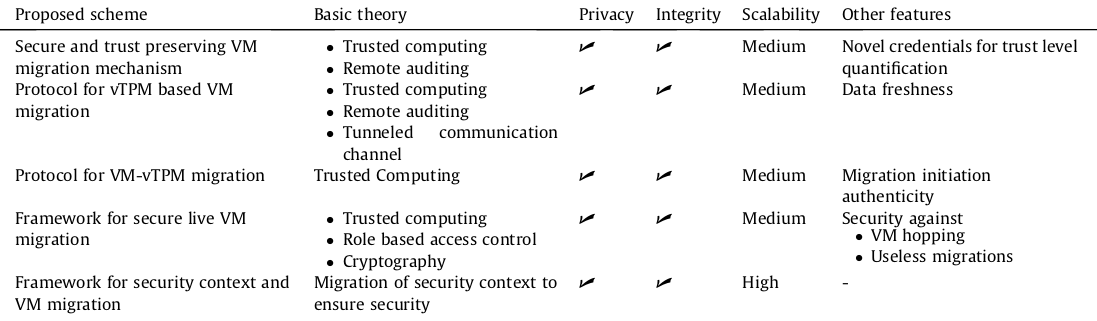
\includegraphics[width=15.5cm]{./pics/VM_migration_tableau.png}
	\caption{Comparaison de diverses solutions permettant une migration de VM sécurisée [\cite{security_cloud_survey}]}
	\label{label-image12}
\end{figure}

\subsection{Partage d'image}
Les images de VM permettent d'initialiser une VM. Pour ne pas corrompre une VM, elle doit être parfaitement intègre et sécurisée. Une fois en place dans le cloud, une VM infectée est capable de gérer son trafic entrant/sortant et peut endommager les données d'autres utilisateurs et créer des problèmes d'intégrité et de confidentialité.
La plupart du temps, les images des VMs sont utilisées par divers utilisateurs et certains utilisateurs malicieux seront tentés d'infecter certaines images en injectant un \textit{malware}. Autre possibilité, un utilisateur malicieux va chercher une faille et un point d'attaque dans le code public des images et si il est capable d'en trouver une, mettre en place une attaque contre ce type d'images. Le tableau comparatif \ref{label-image12} présente diverses solutions garantissant l'utilisation d'images sécurisées de VM. Ce tableau comparatif révèle que la solution \textit{EVDIC} est la plus adéquate. C'est la seule solution permettant une intégrité et une confidentialité des données. En terme de sécurité, il est préférable de protéger les données et de les préserver. On observe que les autres solutions apportent différentes fonctionnalités, mais dans le cadre d'un cloud public, la solution \textit{EVDIC} paraît la plus apte.

\begin{figure}[h]
	\center
	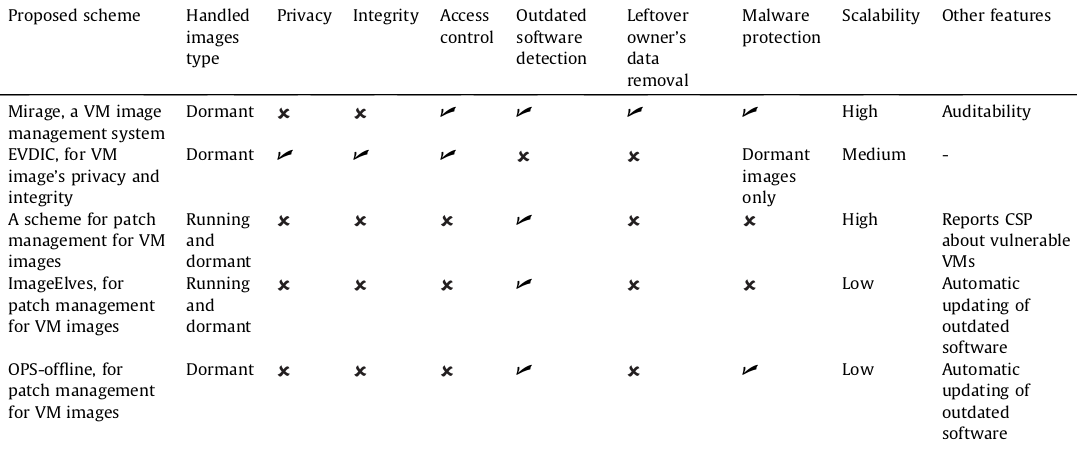
\includegraphics[width=15.5cm]{./pics/securing_VM_images_tableau.png}
	\caption{Comparaison de diverses solutions offrant des images de VM sécurisée [\cite{security_cloud_survey}]}
	\label{label-image13}
\end{figure}

\subsection{Exécution}
Lors de l'exécution d'une VM, cette dernière doit pouvoir offrir des garanties sur la sécurité de son environnement. Premièrement, l'isolation des VMs les unes des autres sur le même matériel (ou \textit{hardware}) physique est obligatoire, car elles sont sujet à des attaques \textit{cross-tenant} ou encore à l'apparition de brèches de données.
Durant l'exécution, des actions sont également sensibles à des attaques. Par exemple, des \textit{rollback} sont possibles sur une VM, mais ils peuvent poser des problèmes de sécurité : des autorisations données à certains utilisateurs non autorisés avant \textit{rollback} ou une modification de la configuration sont des exemples de problèmes de sécurité générés par des \textit{rollback}.
Le tableau comparatif \ref{label-image14} présente diverses solutions permettant de sécuriser l'exécution d'une VM.
Dans la continuité de nos propos, la solution \textit{HyperCoffer} est la plus adaptée à sécuriser l'exécution d'une VM. La séparation de la sécurité et du management des VMs couplée au cryptage des données assure une sécurité satisfaisante pour l'exécution d'une VM. Ce cryptage doit rester interne à la VM, car les données échangées dans le réseau virtuel doivent être en claires. Nous reviendrons sur ce point dans la section~\ref{sec:intra_cloud}. Enfin, en plus de fournir une haute scalabilité, elle permet d'effectuer des \textit{rollbacks} sécurisés.

\begin{figure}[h]
	\center
	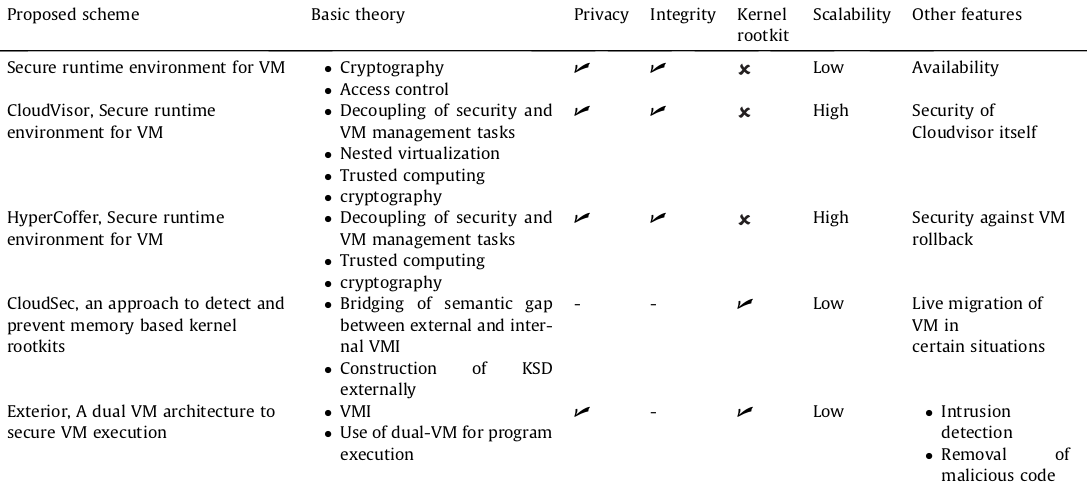
\includegraphics[width=15.5cm]{./pics/security_execution_VM_tableau.png}
	\caption{Comparaison de diverses solutions garantissant une exécution sécurisée d'une VM [\cite{security_cloud_survey}]}
	\label{label-image14}
\end{figure}

\subsection{Sécurité de l'hyperviseur}
Si l'\gls{hyperviseur}, appelé aussi \textit{Virtual Machine Monitor} (ou VMM) est compromise, toutes les VMs contrôlées par la VMM sont alors sous le contrôle d'une personne malveillante. En effet, une VMM tourne en mode privilégié. Si une VMM est compromise, un utilisateur malveillant est capable de s'attribuer des droits non autorisés. C'est pourquoi, notamment, les données des VMs transitant par la VMM sont en position critique posant des problèmes de confidentialité et d'intégrité. Le tableau comparatif \ref{label-image15} présente diverses solutions garantissant la sécurité de l'hyperviseur. Pour ce dernier tableau comparatif, on retiendra \textit{DeHype}. La protection des VMs est assurée. Cette solution sépare également la VMM et le système d'exploitation donnant lieu à un risque d'attaque amoindri provenant du système d'exploitation. Enfin, la réduction des droits privilégiés freine fortement les actions possibles si la VMM est sous le contrôle d'une personne malveillante. 

\begin{figure}[h]
	\center
	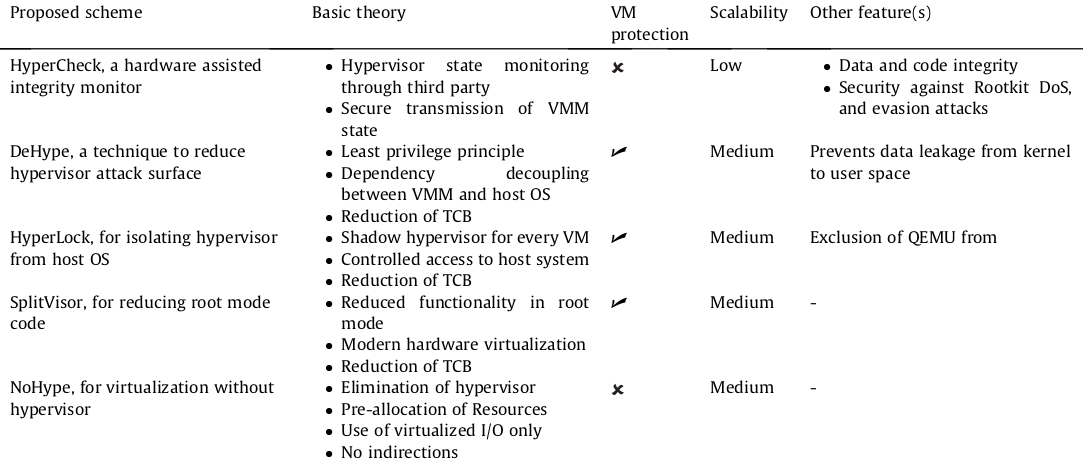
\includegraphics[width=15.5cm]{./pics/VMM_solutions_tableau.png}
	\caption{Comparaison de diverses solutions garantissant la sécurité de l'hyperviseur [\cite{security_cloud_survey}]}
	\label{label-image15}
\end{figure}

\section{Authentification et contrôle d'accès}\label{sec:auth}

Comme précédemment, le CSA (\cite{security_guidelines}) recommande certaines mesures de sécurité. Tout d'abord, l'utilisation de standards libre (OAuth, SAML \cite{security_guidelines}) est recommandée. Deuxièmement, les sources des attributs doivent être aussi proche possible de la \textit{master} source et les attributs doivent être validés par le \textit{master} ou équivalent. Troisièmement, les caractéristiques des entités doivent avoir un niveau de confiance identifié. Quatrièmement, une confiance bi-directionnelle est souhaitée entre deux entités afin d'avoir une relation et des transactions sécurisées. Enfin, les services doivent avoir la capacité d'exporter/importer avec des standards (\gls{XACML} \cite{xacml} \cite{security_guidelines}). 
\newline
La solution retenue pour cette gestion d'identité et ce contrôle d'accès est \textit{Hierarchical Attribute-Set-Based Encryption} (HASBE)\cite{hasbe}. Tout d'abord, elle a été retenue, car elle respecte les recommandations proposées par le CSA. De plus, dans l'étude effectuée \cite{security_cloud_survey}, un tableau comparatif des solutions de gestion d'identité et de contrôle d'accès permet de constater que c'est HASBE qui offre le plus de sécurité tout en offrant une scalabilité performante.
\newline
Pour introduire HASBE, il faut évoquer \textit{Attribute Based Encryption} (ABE) \cite{asb} qui a été utilisé pour fournir un contrôle d'accès dans un environnement cloud. Les messages encryptés sont associés aux attributs des utilisateurs. Ainsi, pour décrypter un message, il est nécessaire que l'utilisateur possède cet attribut. Puis, une extension de ABE, appelée \textit{Attribute Set Based Encryption} (ASBE) \cite{asbe} a introduit un arrangement récursif des attributs en les séparant par catégories permettant à l'utilisateur de pouvoir appliquer des contraintes dynamiques sur la manière dont les attributs remplissent la politique de contrôle d'accès. Enfin, HASBE, étant une extension de ASBE, pose une structure hiérarchique des utilisateurs en introduisant des autorités de confiance et des autorités de domaine. La figure \ref{label-image2} démontre le fonctionnement de HASBE. L'autorité de confiance administre les autorités de domaine qui gèrent à leur tour des autorités de domaine au niveau suivant ou des utilisateurs du domaine. L'autorité de confiance génère et délivre les paramètres systèmes (permettant de créer des groupes notamment) et la clé racine aux autorités de domaine. Les clés sont générées à l'aide de groupes multiplicatifs bilinéaires et les clés asymétriques sont délivrées aux utilisateurs par les autorités de domaine. Ces clés asymétriques sont des \textit{Tree structure based key} c'est-à-dire des structures d'arborescentes hiérarchiques ou chaque élément étant un attribut ou un ensemble d'attribut. Le contrôle d'accès est défini comme une arborescence hiérarchique et il est assuré uniquement pour les données dans le cloud. Enfin, les données sont cryptées avec une clé de cryptage, clé protégée avec le HASBE utilisant la structure d'accès des clés qui spécifie les politiques et attributs de contrôle d'accès. L'accès au déchiffrement est possible pour les utilisateurs possédant les attributs et les accès dans la structure des clés d'accès.
HASBE a été retenue pour couvrir la sécurité de l'authentification et du contrôle d'accès. HASBE fournit un chiffrement par attributs, un accès aux données contrôlée et une mise en place d'une hiérarchie de confiance. Supportant une haute scalabilité, HASBE se voit être la meilleure solution pour répondre à l'hypothèse d'authentification sécurisée de plusieurs acteurs d'un même système.

\begin{figure}[hb]
	\center
	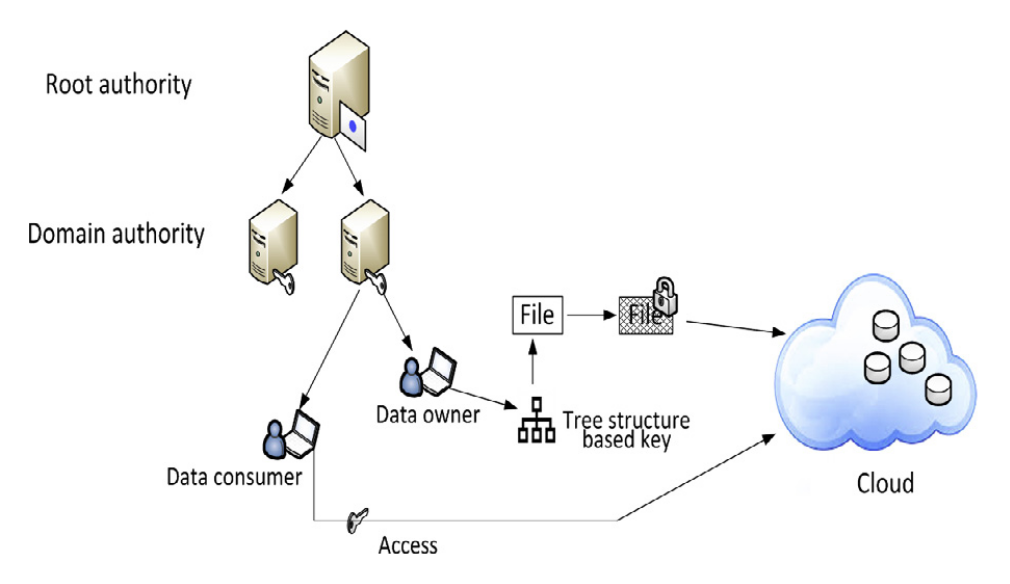
\includegraphics[height=7.5cm]{./pics/hasbe.png}
	\caption{Fonctionnement de HASBE[\cite{security_cloud_survey}]}
	\label{label-image2}
\end{figure}
